\documentclass[conference,letterpaper]{IEEEtran}
\usepackage{cite}
\usepackage{graphicx}
\usepackage{booktabs,array}
\usepackage{microtype}
\usepackage{url}
\setlength{\tabcolsep}{4pt}
\newcolumntype{L}[1]{>{\raggedright\arraybackslash}p{#1}}
\newcommand{\state}[1]{\texttt{#1}}
\title{Effect-Based Bidirectional Authorization for\protect\\Model Context Protocol Tool Use}
% Blank author, affiliation and email spaces retained at the authors' request.
\author{\IEEEauthorblockN{\rule{0pt}{12pt}\hspace{2.7in}}
\IEEEauthorblockA{\rule{0pt}{11pt}\hspace{2.7in}\\
\rule{0pt}{11pt}\hspace{2.7in}\\
\rule{0pt}{11pt}\hspace{2.7in}}}
\begin{document}
\maketitle

\begin{abstract}
Tool-using language-model agents can express the same harmful effect through different tools, routes, and argument encodings. A request filter also leaves a second boundary exposed: an authorized server response may disclose sensitive data or influence later actions. This paper presents an effect-based, bidirectional reference monitor for Model Context Protocol (MCP) interactions. The design combines canonical resource and effect resolution, deterministic restrictive policy, short-lived single-use human approval, governed results, and coverage derived from evidence of exclusive mediation. A TypeScript and PostgreSQL prototype implements durable approval consumption and conservative recovery without retrying an ambiguously forwarded request. Local verification comprises 295 unit tests, 66 integration tests, and four browser workflows, with three fixture-resolved representations receiving the same destructive-action decision and concurrent database consumers creating one forwarding-attempt record. Retained interoperability evidence covers two locally launched open-source MCP servers. These results establish bounded conformance evidence rather than empirical attack-prevention rates. Semantic resolver correctness, adaptive attacks, human approval quality, and production isolation remain unvalidated; deployment coverage therefore remains unprotected. The study identifies how exact execution bindings and conservative coverage reporting can complement effect-level authorization without treating model confidence or prior behavior as authority.
\end{abstract}
\begin{IEEEkeywords}
MCP, AI agent security, reference monitor, authorization, prompt injection, human approval
\end{IEEEkeywords}

\section{Introduction}
Language-model agents increasingly invoke tools that read files, modify repositories, query databases, and contact external services. MCP standardizes how clients discover and invoke these capabilities~\cite{mcp2025}. Interoperability, however, does not establish that an intended action is authorized, that a tool description is truthful, or that returned content is safe to release. Indirect prompt injection can move attacker instructions from retrieved data into the agent's subsequent behavior~\cite{greshake2023}. Consequently, authorization must remain effective even when the model proposes an unsafe call.

Consider an agent asked to summarize a workspace. A poisoned tool result suggests deleting an unrelated file. A tool-name rule may deny a file-removal API while permitting a shell or workspace-management tool that reaches the same object. An approval for one request can also become unsafe if its route, arguments, identity, or policy changes before execution. Finally, a gateway can correctly reject every mediated request while an agent uses a direct credential or native shell to bypass it. These are separate failures of semantic resolution, execution binding, and deployment scope.

Classical protection principles favor complete mediation, least privilege, and fail-safe defaults~\cite{saltzer1975}. Recent agent work already applies external privilege control~\cite{progent2026}. The research problem here is therefore narrower than introducing another proxy: can heterogeneous MCP operations be reduced to a stable effect-level policy while preserving exact invocation identity, governing results, and refusing unsupported protection claims?

This paper makes three contributions. First, it specifies an authorization model that separates semantic equivalence from exact execution bindings, permitting consistent effect-level decisions without making approvals transferable between routes. Second, it describes a bidirectional implementation with transactional single-use approval, result governance, restart recovery, and evidence-scoped coverage. Third, it presents reproducible local verification and explicitly distinguishes executable assertions, actual disposable workflows, and retained third-party interoperability observations.

The contribution is a design and verification study. We do not report a comparative attack-success reduction, a production latency improvement, or universal resistance to prompt injection. Local feature completion does not establish deployment protection: the default runtime remains \state{UNPROTECTED}, and protected production forwarding is disabled.

\section{Background and Related Work}
MCP exposes protocol lifecycle, discovery, tools, resources, and content exchange through structured messages~\cite{mcp2025}. A successfully negotiated session establishes a communication context; it does not authorize every subsequent effect. Likewise, discovery filtering determines what a client can see, but current policy and route integrity must still be checked when a call arrives.

Saltzer and Schroeder's protection principles~\cite{saltzer1975} motivate a monitor outside the agent, explicit authority, and checks at each relevant access. Greshake \emph{et al.}~\cite{greshake2023} show why content from the external environment must not become trusted control input. AgentDojo~\cite{agentdojo2024} operationalizes this distinction by evaluating legitimate utility and targeted attack success separately. Its methodology motivates inspecting intermediate actions rather than treating a correct final answer as evidence of a safe trajectory.

Progent~\cite{progent2026} checks tool names and typed arguments against symbolic rules. An SMT-based comparison determines whether a proposed policy update removes permissions or expands them; expansion passes through a configurable approver. Its approver can involve a human, deny expansion, or accept it automatically. This is substantial prior work on external enforcement. Our approval instead authorizes one bound invocation, not an expansion of the agent's policy.

MCIP~\cite{mcip2025} records MCP interactions as contextual information flows and uses those trajectories to develop risk categories, training data, and a learned safety guard. It motivates tracking what crosses the client--server boundary and why. The present study asks a different operational question: after a request has been resolved, does durable authority remain bound to its resource, effect, and exact invocation? We have not reproduced MCIP or Progent, so this comparison identifies mechanisms to investigate rather than measured advantages.

Table~\ref{tab:related} summarizes emphasis rather than asserting that another system lacks an unreported feature. Our design combines a canonical effect policy with exact, nontransferable execution authority and bidirectional result handling. This integration is complementary to existing guards and sandboxing; comparative superiority requires experiments beyond those reported here.

\begin{table}[t]
\caption{Related Work and the Boundary Studied Here}
\label{tab:related}
\centering\footnotesize
\begin{tabular}{L{.25\columnwidth}L{.66\columnwidth}}
\toprule
Work & Principal emphasis relevant to this study \\
\midrule
AgentDojo~\cite{agentdojo2024} & Agent tasks, injection attacks, and separate utility/security evaluation. \\
Progent~\cite{progent2026} & Symbolic tool policy, SMT comparison, and configurable expansion approval. \\
MCIP~\cite{mcip2025} & Contextual-flow trajectories, risk taxonomy, and learned safety guarding. \\
This work & Canonical effects, exact approval consumption, governed results, and scoped coverage; local conformance evidence. \\
\bottomrule
\end{tabular}
\end{table}

\section{Threat Model and Authorization Properties}
\subsection{Assets, Adversary, and Assumptions}
Protected assets include files, databases, credentials, downstream accounts, route registrations, policy versions, approvals, and audit state. The adversary may influence agent input, tool descriptions, arguments, retrieved data, server results, or errors. It may replay requests, alter route representations, exploit concurrency, induce retries, or attempt cross-session access. A legitimate but mistaken agent is also within scope.

The trusted computing base comprises the gateway runtime, identity and administrative registries, policy engine, category resolvers, approval channel, PostgreSQL, and deployment controls. Correct parsing is not inferred from model confidence. The gateway assumes that trusted resolvers accurately map supported requests to resources and effects, and that independent controls prevent direct access when an enforced deployment is claimed. A compromised operating system, database administrator, or trusted resolver lies outside the guarantees established by local tests.

MCP mediation cannot stop a malicious server from independently abusing privileges it already possesses. It can restrict requests and returned data at its own boundary. Native shell, browser, filesystem, and direct network operations are outside that boundary unless independently constrained. Resource identity can also change after resolution; stable handles, downstream authorization, or an equivalent external binding are needed to address residual time-of-check/time-of-use risk.

\subsection{Semantic Equivalence and Exact Identity}
Let normalization of request \texttt{q} in authenticated context \texttt{c} produce a semantic tuple \texttt{s} and an exact binding \texttt{b}. The tuple contains the resolved resource set, effect, environment, data flow, and risk-relevant parsing and reversibility evidence. The binding records identity, session, request, route, server, tool, schema digest, argument digest, call chain, and policy version. Thus, two equivalent effects need not have identical action hashes. For a fixed policy version, equal semantic tuples must receive the same semantic policy disposition. The final decision then joins that disposition with binding and coverage restrictions, selecting the most restrictive result in the order Deny, RequireApproval, Sandbox, AllowConstrained, Allow. Incompatible constraints or sandbox profiles resolve to denial. Semantic equivalence does not transfer approval: a route-specific restriction may strengthen the final result.

Unsupported syntax, partial analysis, ambiguous resources, and unresolved effects cannot be classified as harmless. Tier~0 is restricted to proven non-sensitive reads; Tier~1 covers bounded reversible writes. Executable or networked operations require stronger controls. Production, destructive, privileged, credential-related, or difficult-to-reverse actions are Tier~3 and require one exact approval or denial. Trust cannot lower this requirement.

\subsection{Execution and Coverage Properties}
For an approval identifier \texttt{a}, the durable coordinator permits at most one forwarding-attempt record. This is an at-most-one initiation property, not exactly-once execution of a remote effect. A lost connection can leave the effect unknown after the approval has been consumed.

Coverage states distinguish \state{ENFORCED}, \state{DEGRADED}, \state{OBSERVE\_ONLY}, and \state{UNPROTECTED}. Enforced coverage requires authenticated, policy-controlled, audited, fail-safe, and exclusive mediation for the exact declared scope. Evidence must be authority-bound, current, and matched to identity, session, route, resource class, and environment. Missing or newer degrading evidence blocks mutations; an older positive assessment is insufficient.

\section{Reference Monitor Design}
Figure~\ref{fig:architecture} shows the request and result paths. The gateway validates inputs, determines authority, and persists security state before effectful execution. Independent operating-system, network, and identity controls remain necessary to close bypass routes. The trust boundary deliberately excludes both agent-generated proposals and server-generated content.

\begin{figure*}[t]
\centering
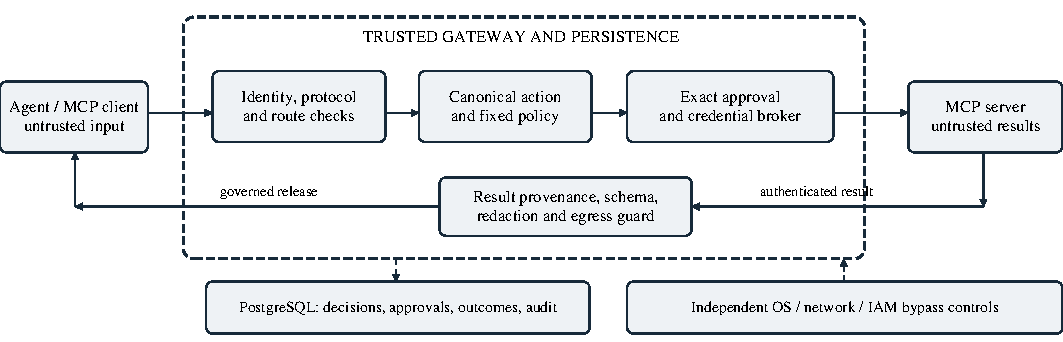
\includegraphics[width=\textwidth]{figures/architecture.pdf}
\caption{Bidirectional mediation. Solid arrows carry requests or governed results; dashed links connect durable security state and independent enforcement evidence. Gateway placement alone does not establish exclusive access to downstream resources.}
\label{fig:architecture}
\end{figure*}

\subsection{Authenticated Discovery and Canonicalization}
Authentication precedes acceptance of model-controlled identity claims. An opaque session binds the authenticated user, agent, client, host, credential identifier, and identity revision. Subsequent requests reauthenticate; another principal cannot select that session by supplying its identifier. Identity rotation invalidates incompatible authority and freezes positive trust evidence.

Administrator-controlled registrations pin server identity, protocol revision, capabilities, credential audience, tool schemas, and route ownership. Duplicate exposed routes are rejected within their scope. Schema or capability drift latches quarantine until administrative review; simply observing the old schema again does not restore authority. Discovery metadata remains untrusted, and every invocation repeats current route and policy checks.

The normalizer recomputes canonical JSON digests and byte counts, verifies the route-selected analyzer, and resolves resources without executing supplied code. Bounded path and URI normalization handles separators, dot segments, percent encoding, and related representation differences. Semantic aliases require a stable resource identity from a trusted resolver. An eleven-category registry validates filesystem, shell, Git, package, network, database, cloud, browser, process, deployment, and MCP-specific analyzer outputs; the registry itself is not a comprehensive parser for those languages.

\subsection{Deterministic Policy and Admission}
Figure~\ref{fig:decision} summarizes the decision flow. Built-in rules, administrative policy, route constraints, and coverage are composed restrictively. A supervisor may contribute adverse evidence, but cannot grant permission or weaken a denial. Unknown operations require approval only where the surrounding guarantees permit it; otherwise they are denied. An absence of suspicious keywords is never sufficient for allowance.

Protocol admission binds request identifiers and nonces to authenticated sessions. Limits cover payloads, results, call depth, delegation, fan-out, retries, concurrency, and time. Cancellation propagates through the execution path, and dependency failures open circuit breakers. A request/action/decision transaction must commit before a decision is exposed to the client or an approval continuation can proceed. PostgreSQL failure has no in-memory runtime fallback.

\begin{figure}[t]
\centering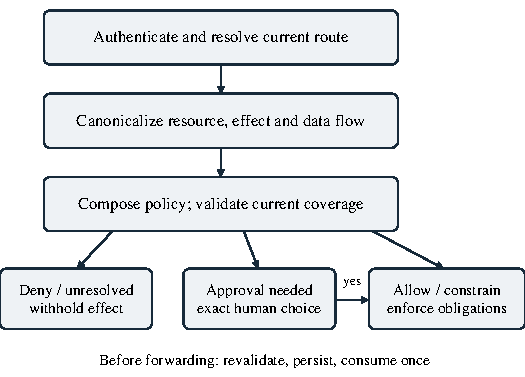
\includegraphics[width=\columnwidth]{figures/decision-flow.pdf}
\caption{Authorization flow. Approval discharges only a matching approval requirement; it cannot bypass denial, current coverage, or execution-time revalidation.}
\label{fig:decision}
\end{figure}

\subsection{Single-Use Approval and Conservative Recovery}
The human interface derives its summary from validated canonical data. It displays the requester, target, route, effect, data flow, risk, reversibility, expiry, coverage, and related attempts. Tier~3 offers only an exact approval or denial. Persistent, wildcard, and bulk grants are invalid. The human authenticates independently of the agent, and browser-origin and CSRF controls protect the decision boundary.

Approval binds the complete invocation, resource and data-flow digests, policy version, and authenticated context for at most five minutes. Figure~\ref{fig:approval} shows durable dispatch and recovery. The human-decision transaction writes both the approved state and a dispatch record. A runtime worker claims the dispatch, reloads authority from PostgreSQL, checks stored invocation, identity, policy, route, schema, and resource bindings, and validates expiry, recorded downstream health, and the latest scoped coverage.

Under a row lock, approval consumption and creation of the unique forwarding-attempt record occur in one transaction. Only its successful consumer may obtain the exact credential lease and invoke the registered forwarder. A losing concurrent request does not reach credential use. Altered arguments, a new route, or a changed policy require a new authorization evaluation and cannot reuse the prior approval.

Figure~\ref{fig:concurrency} separates the database race from the remote effect. The winning transaction creates authority for one initiation; it does not establish exactly-once execution at the server.
\begin{figure*}[t]
\centering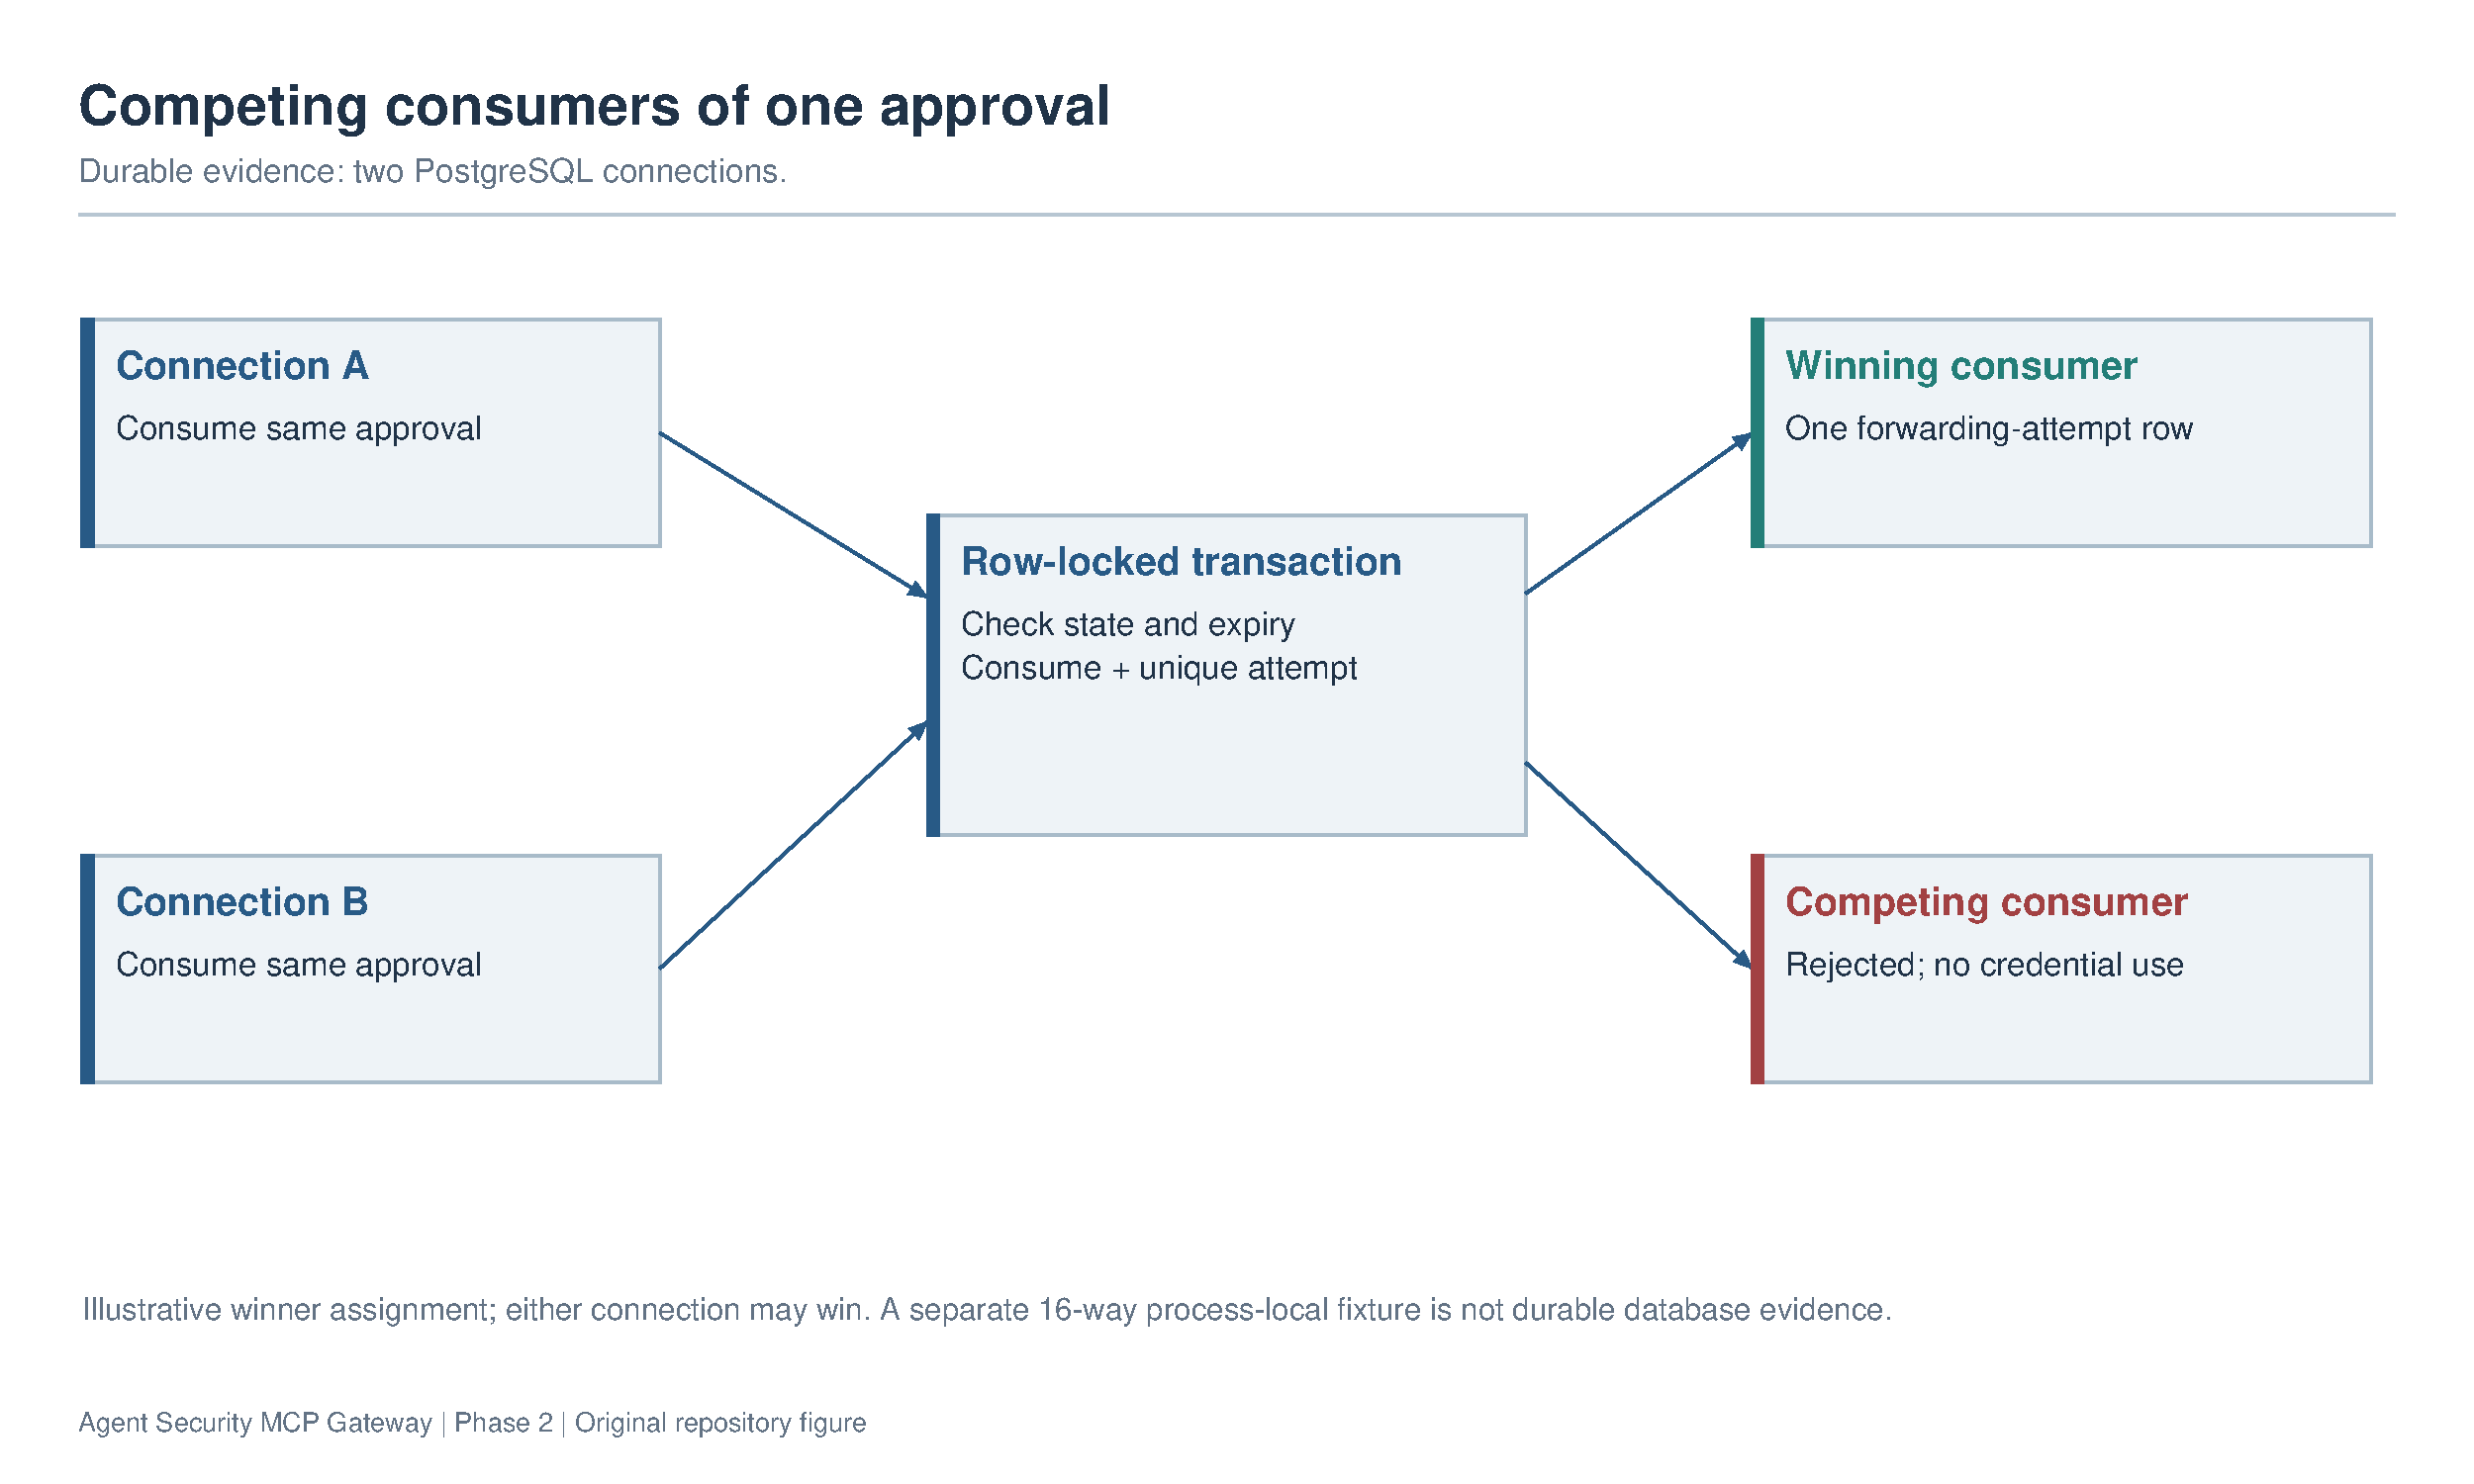
\includegraphics[width=.94\textwidth,trim=0 55 0 15,clip]{../images/09-approval-concurrency.pdf}
\caption{Two consumers compete for one approval. Row locking and the unique forwarding-attempt binding permit one consumer to proceed; the rejected consumer never reaches credential use. This depicts the disposable two-connection test, not an attack-population success rate.}
\label{fig:concurrency}
\end{figure*}

Restart recovery distinguishes uncertainty from failure before execution. A stale unconsumed approval is revoked without forwarding. A consumed attempt lacking a durable outcome becomes \state{UNKNOWN}, records possible partial effects, and is never automatically retried. Concurrent recovery workers use row locking with \state{SKIP LOCKED}; their claim timeout must exceed the bounded executor timeout. This preserves conservative semantics across process interruption without pretending the database and a remote server share one transaction.

\begin{figure}[t]
\centering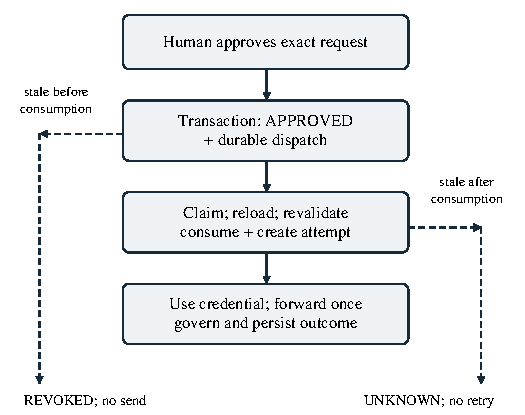
\includegraphics[width=\columnwidth]{figures/approval-flow.pdf}
\caption{Durable approval continuation. Dashed paths show stale-dispatch recovery. Consumption allows one gateway initiation; uncertain downstream effects require investigation rather than automatic retry.}
\label{fig:approval}
\end{figure}

\subsection{Credential Custody and Result Governance}
Credential leases bind the approved action, forwarding attempt, route, audience, endpoint, session, and expiry. Credential material is accessible only inside a non-exporting HTTP sink; redirects are refused. The broker supports a version-pinned HashiCorp Vault KV~v2 adapter, with explicit loopback-only exceptions for disposable tests. Provider or binding failure does not reactivate a consumed approval.

The result boundary binds authenticated server identity, request, action, route, schema, session, and call chain before release. Schema and size checks precede data-egress decisions and known-secret redaction. Dispositions include release, redaction, quarantine, and denial. Raw downstream errors are suppressed, while correlation and outcome information remain available. Returned instructions are marked as untrusted data; the marker is provenance, not proof that a model will ignore the content.

Request authorization and result release are separate decisions. A permitted query may still return prohibited data, and a malformed response can be quarantined even after the remote operation succeeds. Result filtering cannot reverse an already executed effect. Consequently, the outcome records both the forwarding history and the release disposition, including uncertainty and recovery classification.

\begin{figure*}[t]
\centering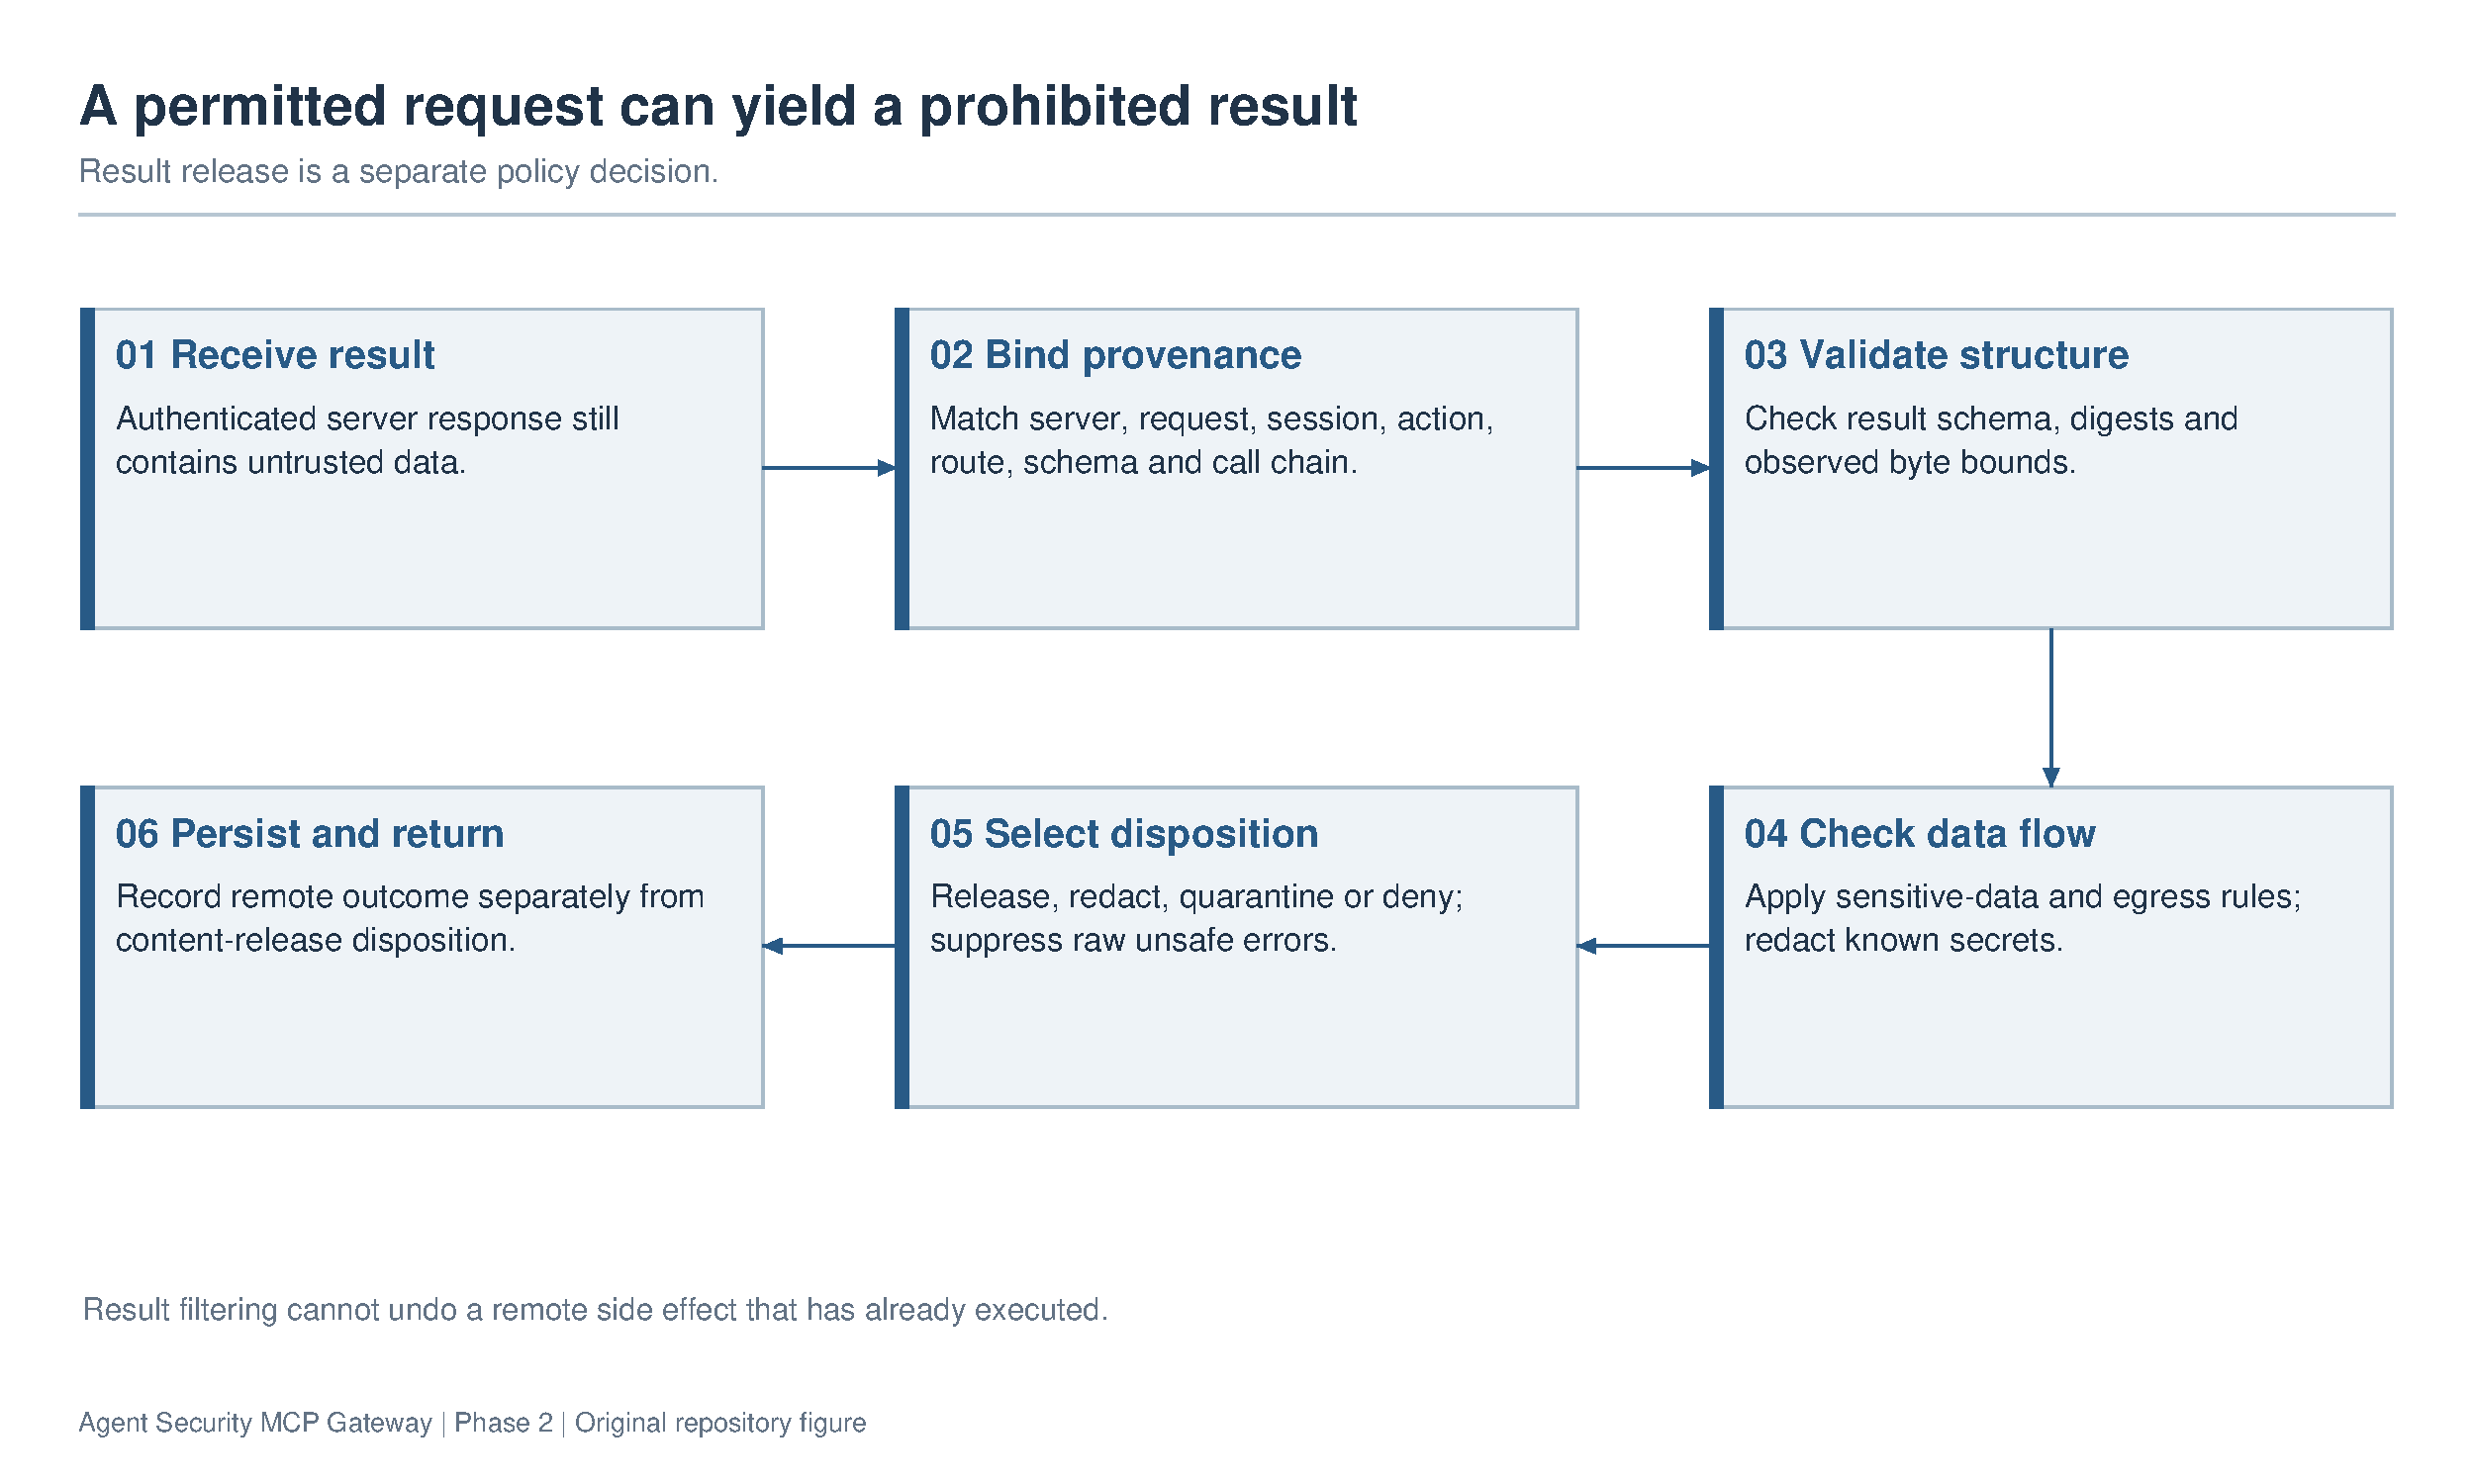
\includegraphics[width=.94\textwidth,trim=0 55 0 15,clip]{../images/11-result-governance.pdf}
\caption{Result governance follows downstream execution. Provenance and structural checks precede data-flow and release decisions; the durable outcome distinguishes a remote effect from whether content was returned. The diagram specifies the boundary and is not a measured detection result.}
\label{fig:results}
\end{figure*}
Figure~\ref{fig:results} makes this second decision explicit: execution permission alone is insufficient to release the response.

\section{Implementation}
The prototype uses strict TypeScript, Express-facing adapters, versioned Zod contracts, and PostgreSQL runtime persistence. Its protocol core pins MCP revision \state{2025-06-18}; compatibility with later revisions is not assumed. Host-neutral modules separate normalization, policy, identity, approval, forwarding, result validation, coverage, and transport. Disposable in-memory implementations support tests, but do not become persistence fallbacks.

The protected identity path verifies mutual TLS and resolves certificate fingerprints through an authoritative PostgreSQL registry. Append-only revisions support rotation and revocation. The approval application loads durable actions and outcomes with server-side scope checks. Missing credential or forwarding dependencies fail startup.

Ordinary audit documents exclude raw arguments and results. Approved continuations retain exact arguments as AES-256-GCM ciphertext with request-bound authenticated data and an external key identifier. The decryption key is not stored in PostgreSQL. Hash-chained events provide tamper evidence within the assumed database trust boundary.

The default loopback entrypoint is intentionally non-forwarding. Separate disposable integration workflows exercise the composed approval executor, credential broker, exact forwarder, and governed outcomes under synthetic scoped enforcement evidence. This distinction permits implementation testing without claiming that production credential custody or direct-path isolation has been established.

A subsequent research extension implements a workspace-file resolver for existing regular files. It accepts registered file tools, trusted workspace aliases, and three precisely specified PowerShell command forms for read, write, and deletion. It inspects filesystem identity and state without executing a supplied command; unsupported syntax, links, hard links, and unsafe paths remain unresolved. Its adapter is restricted to test filesystem routes and is not connected to a protected runtime entrypoint. The retained state digest describes an observation, not a race-free guarantee for a later operation.

Dynamic trust remains a shadow experiment. Its recorded effective decision must equal deterministic policy; a counterfactual cannot authorize Tier~3, override a denial, repair unknown parsing, or restore degraded coverage. The optional supervisor receives minimal redacted context and can only recommend stronger restriction. Neither component is a root of authority.

\section{Local Verification and Results}
\subsection{Questions and Method}
We evaluate three bounded questions: (RQ1) do supported fixture-resolved equivalents preserve the destructive-action policy; (RQ2) do approval, restart, and result boundaries preserve exact request authority; and (RQ3) what does local interoperability establish about deployment scope? The experimental units are automated test cases and explicitly identified disposable workflows, not independent adversarial agent campaigns.

The source baseline is revision \texttt{a887ce725d36}. Fresh validation on September~25, 2026, used Windows x64, Node.js~24.19.0, and Vitest~4.1.11. The procedure builds, lints, type-checks, executes the unit, integration, and browser suites, and validates feature records. Tests use disposable PostgreSQL~18.4, loopback HTTP peers, fixture identities, and injected clocks or resolvers where required. Browser scenarios use Chromium and PostgreSQL with disposable endpoints; the Vault HTTP response is injected in that suite, so it is not a live Vault-service benchmark.

Table~\ref{tab:results} separates fresh regression evidence from retained interoperability observations dated September~20, 2026. It reports no security percentage inferred from the number of passing tests. Tests encode expected behavior and share fixtures; treating them as independent samples of an attack population would produce misleading confidence estimates.

\begin{table}[t]
\caption{Local Verification Evidence and Its Scope}
\label{tab:results}
\centering\footnotesize
\begin{tabular}{L{.31\columnwidth}L{.60\columnwidth}}
\toprule
Evidence & Observation and interpretation \\
\midrule
Unit suite & 295 tests, 32 files; regression and contract checks. \\
Integration suite & 66 tests, 15 files; disposable database and transport boundaries. \\
Browser suite & Four Chromium scenarios; local approval and outcome workflows. \\
Canonical equivalence & Three resolver-backed variants; same DELETE resource, Tier~3, approval required. \\
Durable consumption & Two concurrent connections; one consumption, one rejection, one forwarding row; replay rejected after reconnect. \\
Restart recovery & Unconsumed approval revoked; consumed ambiguous attempt becomes UNKNOWN without retry. \\
Everything MCP [a] & Version 2026.8.31; 13 tools; harmless call completed, unknown tool rejected. \\
Playwright MCP [a] & Version 0.0.81; 26 tools; loopback browser call completed, unknown tool rejected. \\
Deployment scope & UNPROTECTED; production forwarding disabled. \\
\bottomrule
\multicolumn{2}{l}{\scriptsize [a] Retained local observations; not independently operated hosts.}
\end{tabular}
\end{table}

\subsection{RQ1: Conditional Representation Invariance}
The canonical-policy fixture expresses one deletion using a file-removal tool, a shell tool, and a workspace-mutation tool. Route-selected trusted resolvers map their arguments to the same canonical resource and destructive effect. All three produce Tier~3 and \state{REQUIRE\_APPROVAL} under the fixture's enforced scope. This tests policy invariance after resolution; it does not prove equivalence recognition for arbitrary shell programs, encodings, symlinks, or server semantics.

\begin{figure*}[t]
\centering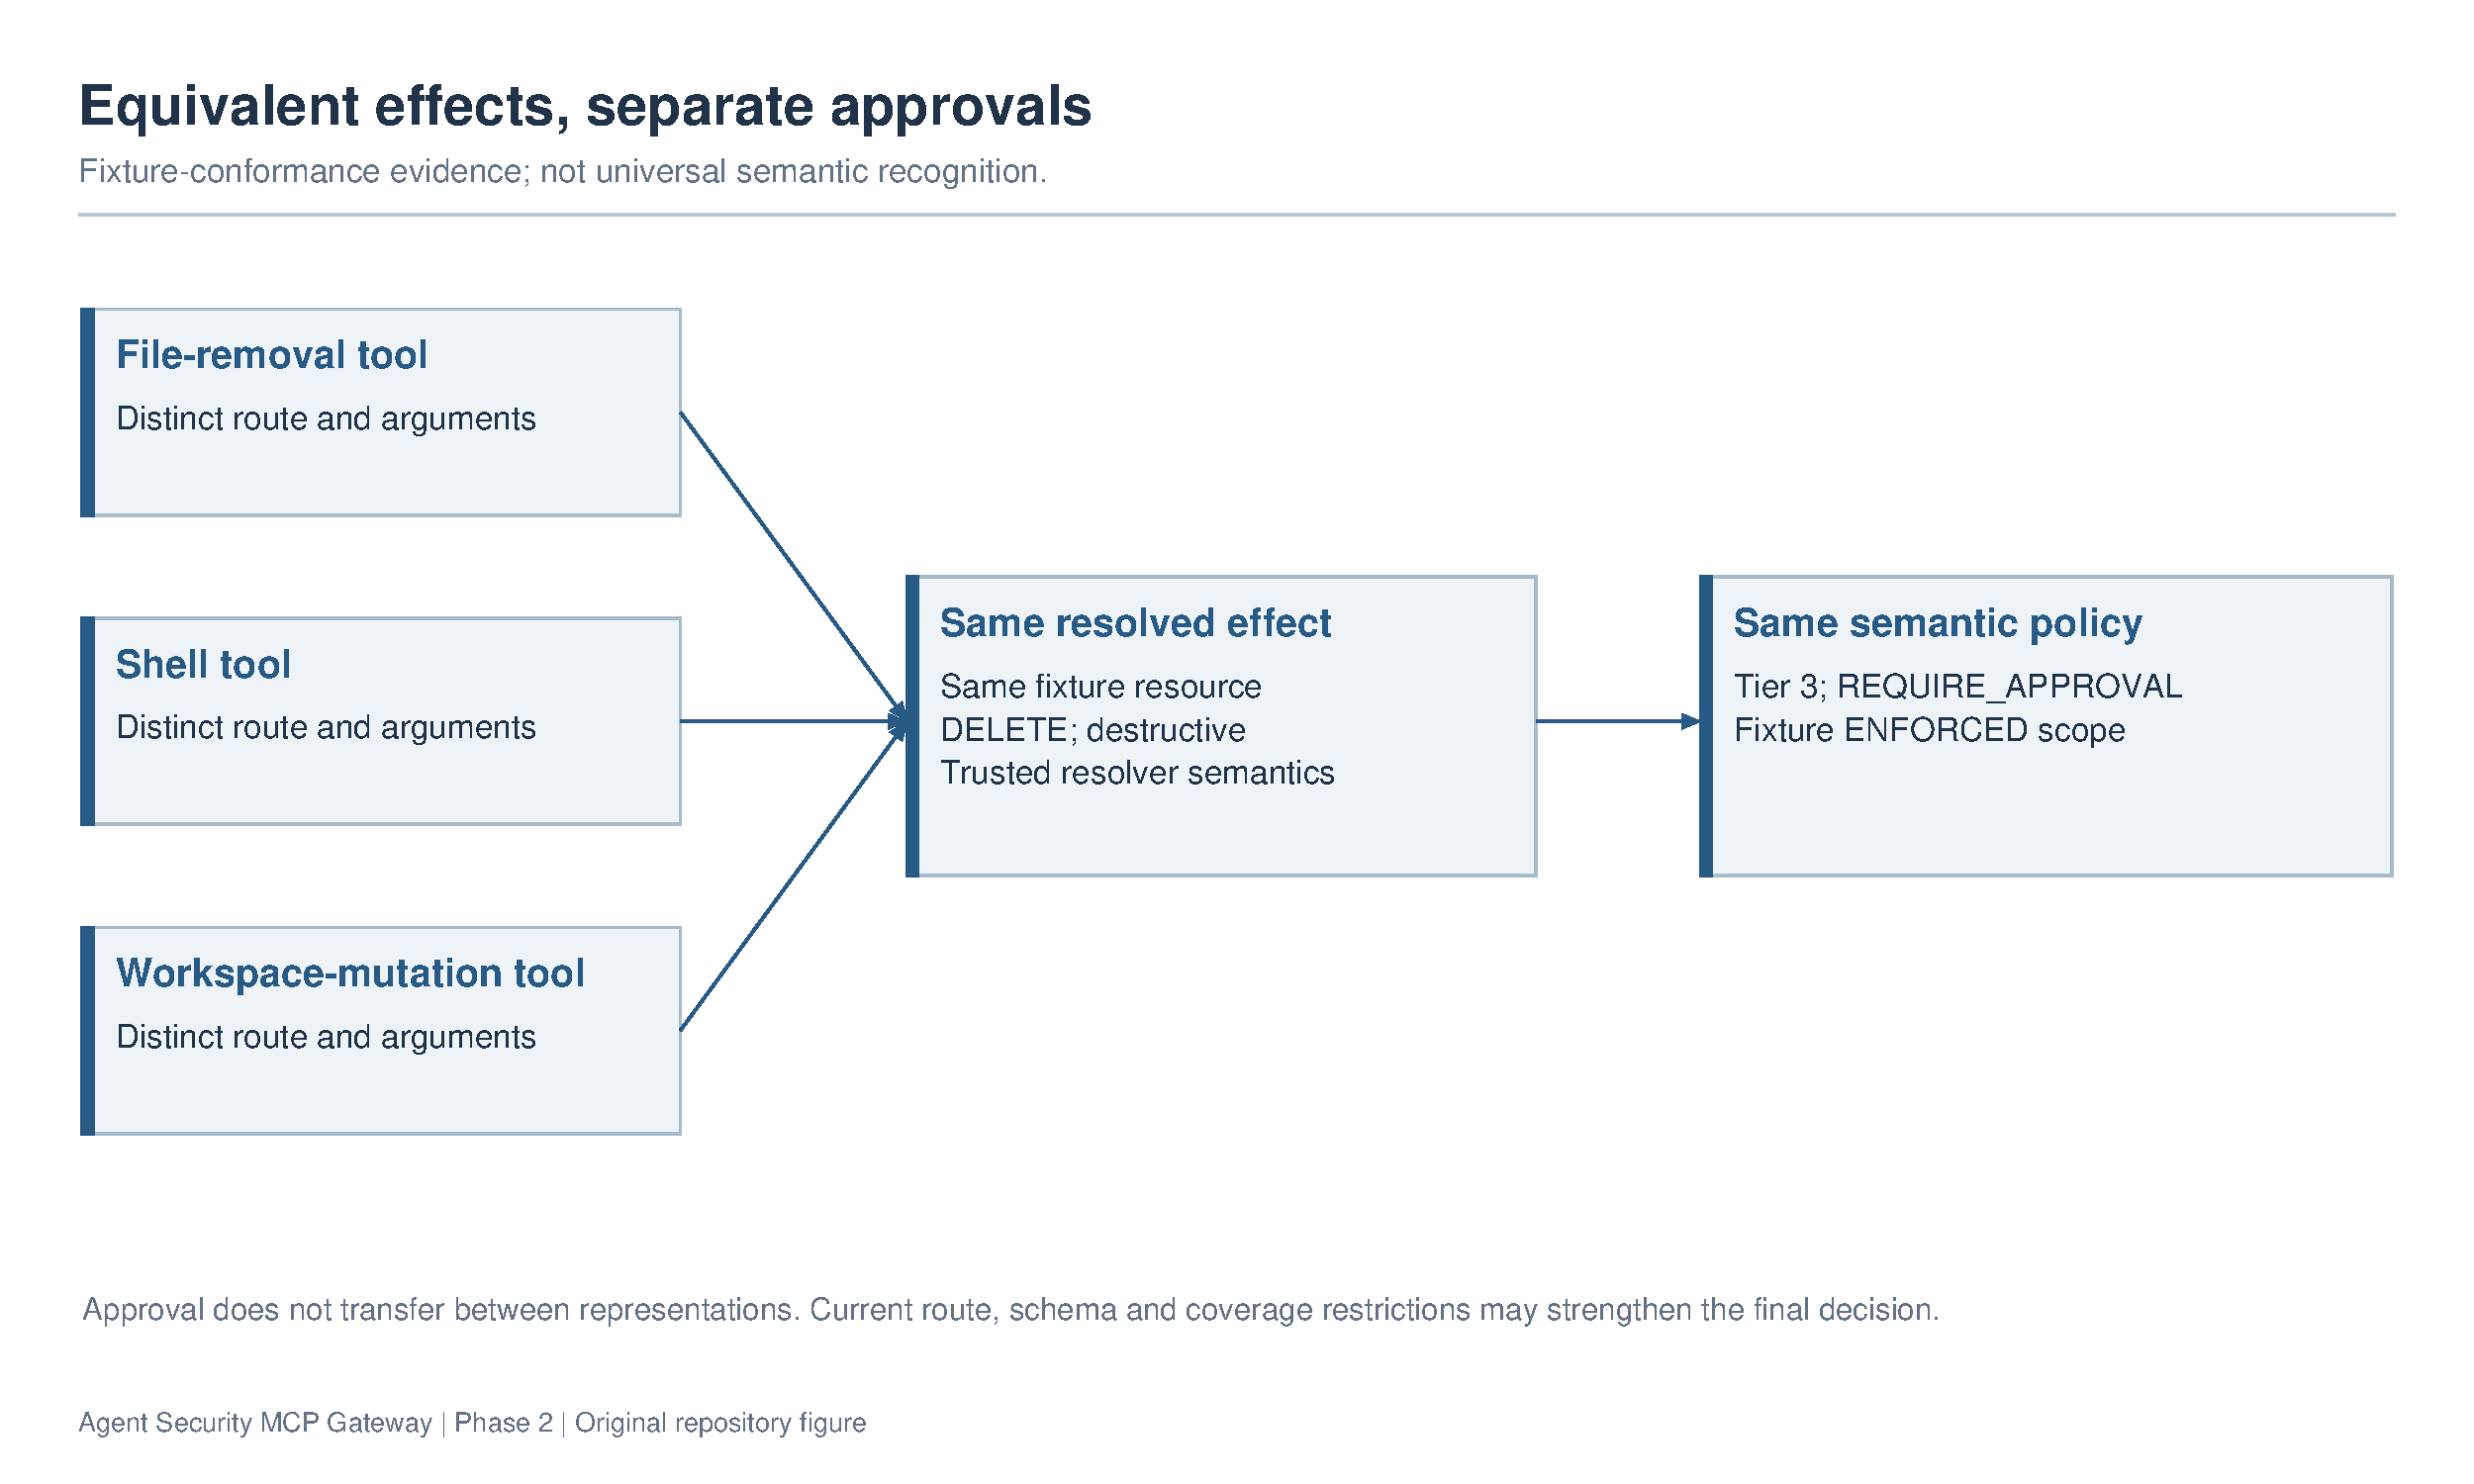
\includegraphics[width=.94\textwidth,trim=0 55 0 15,clip]{../images/05-representation-invariance.pdf}
\caption{Three fixture-resolved representations share a resource and destructive effect, so semantic policy agrees. Exact route and argument bindings remain distinct: approval for one invocation does not authorize the others.}
\label{fig:equivalence}
\end{figure*}
Figure~\ref{fig:equivalence} illustrates this conditional result and the boundary between equivalent policy and transferable authority.

Additional assertions reject missing analyzers, category mismatch, partial parsing, and conflicting sandbox profiles. Non-read actions are denied under degraded, observe-only, and unprotected coverage. These checks support fail-closed treatment of unresolved cases, but the registry's strictness must not be confused with completeness of the semantic analyzers it hosts.

The subsequent resolver extension has a development corpus of 50 calls: 24 benign and 26 adversarial scenarios in 30 families. Every label is marked \state{CANDIDATE\_UNREVIEWED}; all families are development data, and none is held out. These counts describe corpus composition, not resolver accuracy or attack prevention. Independent semantic review, untouched evaluation families, and an observer of executed effects are still needed. The September~25 regression counts above precede this extension and are not its validation results.

\subsection{RQ2: Exact Authority Across Failure Boundaries}
The PostgreSQL race uses two consumers on separate connections. One atomically consumes approval and creates the forwarding record; the other is rejected. Reopening the store does not permit replay. A separate process-local approval fixture exercises a 16-way attempt race, but the two-connection result is the relevant durable database evidence.

Integration workflows connect approval to a disposable credentialed HTTP request, governed result, provenance, and persisted outcome. They check argument substitution, provenance mismatch, secret redaction, quarantine, byte bounds, cancellation, and redirect refusal. Newer unprotected coverage defeats older enforced evidence before forwarding. Table~\ref{tab:failures} links representative failure triggers to observed safe behavior.

\begin{table}[t]
\caption{Representative Failure Cases Exercised Locally}
\label{tab:failures}
\centering\footnotesize
\begin{tabular}{L{.40\columnwidth}L{.51\columnwidth}}
\toprule
Trigger & Required and tested behavior \\
\midrule
Changed arguments or route & Reject the prior execution binding. \\
Consumed approval replay & Deny; do not create another attempt. \\
New coverage degradation & Reject mutation before credential use. \\
Stale unconsumed dispatch & Revoke; create no forwarding attempt. \\
Consumed dispatch, no outcome & Record UNKNOWN and partial-effect risk; never retry. \\
Invalid result provenance/schema & Withhold or quarantine the result. \\
Known secret in returned content & Redact or withhold before release. \\
Required persistence unavailable & Fail closed; no memory fallback. \\
\bottomrule
\end{tabular}
\end{table}

Four browser scenarios passed, covering denial; a governed approve-once workflow; expiry, stale authority, and coverage changes; and provider or result failures. Reload and competing tabs exercise durable state rather than client-side button state. These scenarios verify application behavior, not human comprehension, decision accuracy, or resistance to approval fatigue.

\subsection{RQ3: Interoperability and Evidence Fidelity}
The retained verifier launches two version-pinned upstream servers locally with sanitized environments and negotiates MCP over stdio. Each lists tools, completes one harmless call, and rejects an unknown tool. The artifact includes package integrity and an evidence digest. This supports compatibility for those selected operations only; it neither exercises independently administered deployments nor establishes comparative defense effectiveness.

The seeded evaluation harness contains 30 attack classes across protocol, policy invariance, malicious content, and human/trust suites. Its 93-record demonstration supplies deterministic expected outcomes and seeded synthetic latency. Similarly, a two-adapter workflow executes six real HTTP initialization requests but supplies policy and timing observations. Both validate harness mechanics. Neither dataset supports attack-success, latency, or usability improvement claims, and neither is presented as an empirical benchmark here.

\section{Discussion and Limitations}
\subsection{What the Evidence Supports}
The strongest local result is compositional: supported policy decisions can be tied to a durable approval, at most one forwarding initiation, and a separately governed result. This makes several failure states explicit that a simple tool-name allowlist would leave unspecified. It also exposes a useful distinction between semantic equivalence and authority identity. Two calls may deserve the same policy while still requiring different approvals because their route or invocation bindings differ.

These properties depend on resolver correctness, current observations, and faithful adapters. The current continuation rechecks stored authority rather than rerunning semantic resolution and policy evaluation; freshness against changed external state requires additional deployment guarantees. Revalidation cannot eliminate all races inside an independently executing downstream system. A result's authenticated provenance identifies its source, not its truthfulness. Known-secret redaction does not prove general non-disclosure, and untrusted-content labels do not guarantee model obedience. The architecture therefore requires least-privilege downstream accounts and external containment alongside the monitor.

\subsection{Threats to Validity and Next Experiments}
Internal validity is limited by fixture-controlled identities, resolvers, coverage, and selected failure schedules. No formal verification or exhaustive state-space exploration is claimed. External validity is limited to the pinned protocol and selected local tools; a different host, schema, resolver, or server behavior may expose additional failures. Local third-party processes do not supply independent security review or independently operated host evidence.

An effectiveness study should pair benign tasks and adaptive attacks across native MCP, deterministic gateway policy, and policy with structured awareness. Attacks should target equivalent effects across routes, alternate encodings, poisoned results, retries, and concurrent approval schedules. Full trajectories must record unsafe intermediate effects even when the final task answer appears correct. Following the separation used by AgentDojo~\cite{agentdojo2024}, task completion under policy and attack success should have distinct denominators; blocked attacks that also prevent legitimate work must not be counted as unqualified success.

The next experiment should report per-condition counts, model and server versions, seeds, defense configuration, and checked outcome labels. Measure admission, database, approval, and result latency separately from human waiting time; measure approval burden, false denials, safe replanning, and human error. Shadow trust should remain observational until paired evidence supports a bounded change without increased unsafe authorization. Current tests use disposable resources, no production credentials, and no human participants; future studies need their own consent, ethics, isolation, and incident-response procedures.

\section{Conclusion}
Effect-based MCP authorization requires both stable semantic decisions and exact execution identity. The presented reference monitor combines deterministic policy, transactionally consumed human approval, conservative recovery, bidirectional result mediation, and evidence-scoped coverage. Local tests support these mechanisms for selected disposable workflows, while retained checks establish limited interoperability with two open-source servers. They do not establish universal parsing, empirical attack prevention, or production protection. The resulting boundary is deliberately explicit: unsupported semantics and missing coverage fail closed, uncertain effects are not retried, and model-derived trust never substitutes for authority.

\bibliographystyle{IEEEtran}
\bibliography{references}
\end{document}
